% XCircuit output "synth_out.tex" for LaTeX input from synth_out.eps
\def\putbox#1#2#3#4{\makebox[0in][l]{\makebox[#1][l]{}\raisebox{\baselineskip}[0in][0in]{\raisebox{#2}[0in][0in]{\scalebox{#3}{#4}}}}}
\def\rightbox#1{\makebox[0in][r]{#1}}
\def\centbox#1{\makebox[0in]{#1}}
\def\topbox#1{\raisebox{-0.60\baselineskip}[0in][0in]{#1}}
\def\midbox#1{\raisebox{-0.20\baselineskip}[0in][0in]{#1}}
   \scalebox{1}{
   \normalsize
   \parbox{5.26562in}{
   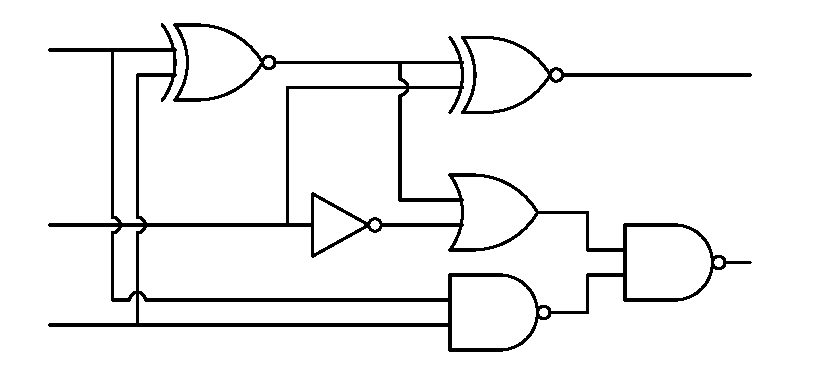
\includegraphics[scale=1]{synth_out.eps}\\
   % translate x=768 y=416 scale 0.38
   \putbox{0.06in}{2.06in}{1.20}{$x$}%
   \putbox{0.06in}{0.89in}{1.20}{$y$}%
   \putbox{0.06in}{0.22in}{1.20}{$z$}%
   \putbox{4.97in}{1.89in}{1.20}{$f$}%
   \putbox{4.97in}{0.64in}{1.20}{$g$}%
   } % close 'parbox'
   } % close 'scalebox'
   \vspace{-\baselineskip} % this is not necessary, but looks better
